\documentclass[11pt,compress,t,notes=noshow, xcolor=table]{beamer}

\documentclass[11pt,compress,t,notes=noshow, xcolor=table]{beamer}
\usepackage[]{graphicx}\usepackage[]{color}
% maxwidth is the original width if it is less than linewidth
% otherwise use linewidth (to make sure the graphics do not exceed the margin)
\makeatletter
\def\maxwidth{ %
  \ifdim\Gin@nat@width>\linewidth
    \linewidth
  \else
    \Gin@nat@width
  \fi
}
\makeatother

\definecolor{fgcolor}{rgb}{0.345, 0.345, 0.345}
\newcommand{\hlnum}[1]{\textcolor[rgb]{0.686,0.059,0.569}{#1}}%
\newcommand{\hlstr}[1]{\textcolor[rgb]{0.192,0.494,0.8}{#1}}%
\newcommand{\hlcom}[1]{\textcolor[rgb]{0.678,0.584,0.686}{\textit{#1}}}%
\newcommand{\hlopt}[1]{\textcolor[rgb]{0,0,0}{#1}}%
\newcommand{\hlstd}[1]{\textcolor[rgb]{0.345,0.345,0.345}{#1}}%
\newcommand{\hlkwa}[1]{\textcolor[rgb]{0.161,0.373,0.58}{\textbf{#1}}}%
\newcommand{\hlkwb}[1]{\textcolor[rgb]{0.69,0.353,0.396}{#1}}%
\newcommand{\hlkwc}[1]{\textcolor[rgb]{0.333,0.667,0.333}{#1}}%
\newcommand{\hlkwd}[1]{\textcolor[rgb]{0.737,0.353,0.396}{\textbf{#1}}}%
\let\hlipl\hlkwb

\usepackage{framed}
\makeatletter
\newenvironment{kframe}{%
 \def\at@end@of@kframe{}%
 \ifinner\ifhmode%
  \def\at@end@of@kframe{\end{minipage}}%
  \begin{minipage}{\columnwidth}%
 \fi\fi%
 \def\FrameCommand##1{\hskip\@totalleftmargin \hskip-\fboxsep
 \colorbox{shadecolor}{##1}\hskip-\fboxsep
     % There is no \\@totalrightmargin, so:
     \hskip-\linewidth \hskip-\@totalleftmargin \hskip\columnwidth}%
 \MakeFramed {\advance\hsize-\width
   \@totalleftmargin\z@ \linewidth\hsize
   \@setminipage}}%
 {\par\unskip\endMakeFramed%
 \at@end@of@kframe}
\makeatother

\definecolor{shadecolor}{rgb}{.97, .97, .97}
\definecolor{messagecolor}{rgb}{0, 0, 0}
\definecolor{warningcolor}{rgb}{1, 0, 1}
\definecolor{errorcolor}{rgb}{1, 0, 0}
\newenvironment{knitrout}{}{} % an empty environment to be redefined in TeX

\usepackage{alltt}
\newcommand{\SweaveOpts}[1]{}  % do not interfere with LaTeX
\newcommand{\SweaveInput}[1]{} % because they are not real TeX commands
\newcommand{\Sexpr}[1]{}       % will only be parsed by R
\newcommand{\xmark}{\ding{55}}%


\usepackage[english]{babel}
\usepackage[utf8]{inputenc}

\usepackage{dsfont}
\usepackage{verbatim}
\usepackage{amsmath}
\usepackage{amsfonts}
\usepackage{amssymb}
\usepackage{bm}
\usepackage{csquotes}
\usepackage{multirow}
\usepackage{longtable}
\usepackage{booktabs}
\usepackage{enumerate}
\usepackage[absolute,overlay]{textpos}
\usepackage{psfrag}
\usepackage{algorithm}
\usepackage{algpseudocode}
\usepackage{eqnarray}
\usepackage{arydshln}
\usepackage{tabularx}
\usepackage{placeins}
\usepackage{tikz}
\usepackage{setspace}
\usepackage{colortbl}
\usepackage{mathtools}
\usepackage{wrapfig}
\usepackage{bm}
\usepackage{amsmath}
\usepackage{pifont}

\usetikzlibrary{shapes,arrows,automata,positioning,calc,chains,trees, shadows}
\tikzset{
  %Define standard arrow tip
  >=stealth',
  %Define style for boxes
  punkt/.style={
    rectangle,
    rounded corners,
    draw=black, very thick,
    text width=6.5em,
    minimum height=2em,
    text centered},
  % Define arrow style
  pil/.style={
    ->,
    thick,
    shorten <=2pt,
    shorten >=2pt,}
}

\usepackage{subfig}

% Defines macros and environments
\usepackage{../../style/lmu-lecture}


\let\code=\texttt
\let\proglang=\textsf

\setkeys{Gin}{width=0.9\textwidth}

\setbeamertemplate{frametitle}{\expandafter\uppercase\expandafter\insertframetitle}

\usepackage{bbm}
% basic latex stuff
\newcommand{\pkg}[1]{{\fontseries{b}\selectfont #1}} %fontstyle for R packages
\newcommand{\lz}{\vspace{0.5cm}} %vertical space
\newcommand{\dlz}{\vspace{1cm}} %double vertical space
\newcommand{\oneliner}[1] % Oneliner for important statements
{\begin{block}{}\begin{center}\begin{Large}#1\end{Large}\end{center}\end{block}}


%new environments
\newenvironment{vbframe}  %frame with breaks and verbatim
{
 \begin{frame}[containsverbatim,allowframebreaks]
}
{
\end{frame}
}

\newenvironment{vframe}  %frame with verbatim without breaks (to avoid numbering one slided frames)
{
 \begin{frame}[containsverbatim]
}
{
\end{frame}
}

\newenvironment{blocki}[1]   % itemize block
{
 \begin{block}{#1}\begin{itemize}
}
{
\end{itemize}\end{block}
}

\newenvironment{fragileframe}[2]{  %fragile frame with framebreaks
\begin{frame}[allowframebreaks, fragile, environment = fragileframe]
\frametitle{#1}
#2}
{\end{frame}}


\newcommand{\myframe}[2]{  %short for frame with framebreaks
\begin{frame}[allowframebreaks]
\frametitle{#1}
#2
\end{frame}}

\newcommand{\remark}[1]{
  \textbf{Remark:} #1
}


\newenvironment{deleteframe}
{
\begingroup
\usebackgroundtemplate{
\includegraphics[width=\paperwidth,height=\paperheight]{../style/color/red.png}}
 \begin{frame}
}
{
\end{frame}
\endgroup
}
\newenvironment{simplifyframe}
{
\begingroup
\usebackgroundtemplate{
\includegraphics[width=\paperwidth,height=\paperheight]{../style/color/yellow.png}}
 \begin{frame}
}
{
\end{frame}
\endgroup
}\newenvironment{draftframe}
{
\begingroup
\usebackgroundtemplate{
\includegraphics[width=\paperwidth,height=\paperheight]{../style/color/green.jpg}}
 \begin{frame}
}
{
\end{frame}
\endgroup
}
% https://tex.stackexchange.com/a/261480: textcolor that works in mathmode
\makeatletter
\renewcommand*{\@textcolor}[3]{%
  \protect\leavevmode
  \begingroup
    \color#1{#2}#3%
  \endgroup
}
\makeatother





% math spaces
\ifdefined\N                                                                
\renewcommand{\N}{\mathds{N}} % N, naturals
\else \newcommand{\N}{\mathds{N}} \fi 
\newcommand{\Z}{\mathds{Z}} % Z, integers
\newcommand{\Q}{\mathds{Q}} % Q, rationals
\newcommand{\R}{\mathds{R}} % R, reals
\ifdefined\C 
  \renewcommand{\C}{\mathds{C}} % C, complex
\else \newcommand{\C}{\mathds{C}} \fi
\newcommand{\continuous}{\mathcal{C}} % C, space of continuous functions
\newcommand{\M}{\mathcal{M}} % machine numbers
\newcommand{\epsm}{\epsilon_m} % maximum error

% counting / finite sets
\newcommand{\setzo}{\{0, 1\}} % set 0, 1
\newcommand{\setmp}{\{-1, +1\}} % set -1, 1
\newcommand{\unitint}{[0, 1]} % unit interval

% basic math stuff
\newcommand{\xt}{\tilde x} % x tilde
\newcommand{\argmax}{\operatorname{arg\,max}} % argmax
\newcommand{\argmin}{\operatorname{arg\,min}} % argmin
\newcommand{\argminlim}{\mathop{\mathrm{arg\,min}}\limits} % argmax with limits
\newcommand{\argmaxlim}{\mathop{\mathrm{arg\,max}}\limits} % argmin with limits  
\newcommand{\sign}{\operatorname{sign}} % sign, signum
\newcommand{\I}{\mathbb{I}} % I, indicator
\newcommand{\order}{\mathcal{O}} % O, order
\newcommand{\pd}[2]{\frac{\partial{#1}}{\partial #2}} % partial derivative
\newcommand{\floorlr}[1]{\left\lfloor #1 \right\rfloor} % floor
\newcommand{\ceillr}[1]{\left\lceil #1 \right\rceil} % ceiling

% sums and products
\newcommand{\sumin}{\sum\limits_{i=1}^n} % summation from i=1 to n
\newcommand{\sumim}{\sum\limits_{i=1}^m} % summation from i=1 to m
\newcommand{\sumjn}{\sum\limits_{j=1}^n} % summation from j=1 to p
\newcommand{\sumjp}{\sum\limits_{j=1}^p} % summation from j=1 to p
\newcommand{\sumik}{\sum\limits_{i=1}^k} % summation from i=1 to k
\newcommand{\sumkg}{\sum\limits_{k=1}^g} % summation from k=1 to g
\newcommand{\sumjg}{\sum\limits_{j=1}^g} % summation from j=1 to g
\newcommand{\meanin}{\frac{1}{n} \sum\limits_{i=1}^n} % mean from i=1 to n
\newcommand{\meanim}{\frac{1}{m} \sum\limits_{i=1}^m} % mean from i=1 to n
\newcommand{\meankg}{\frac{1}{g} \sum\limits_{k=1}^g} % mean from k=1 to g
\newcommand{\prodin}{\prod\limits_{i=1}^n} % product from i=1 to n
\newcommand{\prodkg}{\prod\limits_{k=1}^g} % product from k=1 to g
\newcommand{\prodjp}{\prod\limits_{j=1}^p} % product from j=1 to p

% linear algebra
\newcommand{\one}{\boldsymbol{1}} % 1, unitvector
\newcommand{\zero}{\mathbf{0}} % 0-vector
\newcommand{\id}{\boldsymbol{I}} % I, identity
\newcommand{\diag}{\operatorname{diag}} % diag, diagonal
\newcommand{\trace}{\operatorname{tr}} % tr, trace
\newcommand{\spn}{\operatorname{span}} % span
\newcommand{\scp}[2]{\left\langle #1, #2 \right\rangle} % <.,.>, scalarproduct
\newcommand{\mat}[1]{\begin{pmatrix} #1 \end{pmatrix}} % short pmatrix command
\newcommand{\Amat}{\mathbf{A}} % matrix A
\newcommand{\Deltab}{\mathbf{\Delta}} % error term for vectors

% basic probability + stats
\renewcommand{\P}{\mathds{P}} % P, probability
\newcommand{\E}{\mathds{E}} % E, expectation
\newcommand{\var}{\mathsf{Var}} % Var, variance
\newcommand{\cov}{\mathsf{Cov}} % Cov, covariance
\newcommand{\corr}{\mathsf{Corr}} % Corr, correlation
\newcommand{\normal}{\mathcal{N}} % N of the normal distribution
\newcommand{\iid}{\overset{i.i.d}{\sim}} % dist with i.i.d superscript
\newcommand{\distas}[1]{\overset{#1}{\sim}} % ... is distributed as ...

% machine learning
\newcommand{\Xspace}{\mathcal{X}} % X, input space
\newcommand{\Yspace}{\mathcal{Y}} % Y, output space
\newcommand{\nset}{\{1, \ldots, n\}} % set from 1 to n
\newcommand{\pset}{\{1, \ldots, p\}} % set from 1 to p
\newcommand{\gset}{\{1, \ldots, g\}} % set from 1 to g
\newcommand{\Pxy}{\mathbb{P}_{xy}} % P_xy
\newcommand{\Exy}{\mathbb{E}_{xy}} % E_xy: Expectation over random variables xy
\newcommand{\xv}{\mathbf{x}} % vector x (bold)
\newcommand{\xtil}{\tilde{\mathbf{x}}} % vector x-tilde (bold)
\newcommand{\yv}{\mathbf{y}} % vector y (bold)
\newcommand{\xy}{(\xv, y)} % observation (x, y)
\newcommand{\xvec}{\left(x_1, \ldots, x_p\right)^\top} % (x1, ..., xp) 
\newcommand{\Xmat}{\mathbf{X}} % Design matrix
\newcommand{\allDatasets}{\mathds{D}} % The set of all datasets
\newcommand{\allDatasetsn}{\mathds{D}_n}  % The set of all datasets of size n 
\newcommand{\D}{\mathcal{D}} % D, data
\newcommand{\Dn}{\D_n} % D_n, data of size n
\newcommand{\Dtrain}{\mathcal{D}_{\text{train}}} % D_train, training set
\newcommand{\Dtest}{\mathcal{D}_{\text{test}}} % D_test, test set
\newcommand{\xyi}[1][i]{\left(\xv^{(#1)}, y^{(#1)}\right)} % (x^i, y^i), i-th observation
\newcommand{\Dset}{\left( \xyi[1], \ldots, \xyi[n]\right)} % {(x1,y1)), ..., (xn,yn)}, data
\newcommand{\defAllDatasetsn}{(\Xspace \times \Yspace)^n} % Def. of the set of all datasets of size n 
\newcommand{\defAllDatasets}{\bigcup_{n \in \N}(\Xspace \times \Yspace)^n} % Def. of the set of all datasets 
\newcommand{\xdat}{\left\{ \xv^{(1)}, \ldots, \xv^{(n)}\right\}} % {x1, ..., xn}, input data
\newcommand{\ydat}{\left\{ \yv^{(1)}, \ldots, \yv^{(n)}\right\}} % {y1, ..., yn}, input data
\newcommand{\yvec}{\left(y^{(1)}, \hdots, y^{(n)}\right)^\top} % (y1, ..., yn), vector of outcomes
\renewcommand{\xi}[1][i]{\xv^{(#1)}} % x^i, i-th observed value of x
\newcommand{\yi}[1][i]{y^{(#1)}} % y^i, i-th observed value of y 
\newcommand{\xivec}{\left(x^{(i)}_1, \ldots, x^{(i)}_p\right)^\top} % (x1^i, ..., xp^i), i-th observation vector
\newcommand{\xj}{\xv_j} % x_j, j-th feature
\newcommand{\xjvec}{\left(x^{(1)}_j, \ldots, x^{(n)}_j\right)^\top} % (x^1_j, ..., x^n_j), j-th feature vector
\newcommand{\phiv}{\mathbf{\phi}} % Basis transformation function phi
\newcommand{\phixi}{\mathbf{\phi}^{(i)}} % Basis transformation of xi: phi^i := phi(xi)

%%%%%% ml - models general
\newcommand{\lamv}{\bm{\lambda}} % lambda vector, hyperconfiguration vector
\newcommand{\Lam}{\bm{\Lambda}}	 % Lambda, space of all hpos
% Inducer / Inducing algorithm
\newcommand{\preimageInducer}{\left(\defAllDatasets\right)\times\Lam} % Set of all datasets times the hyperparameter space
\newcommand{\preimageInducerShort}{\allDatasets\times\Lam} % Set of all datasets times the hyperparameter space
% Inducer / Inducing algorithm
\newcommand{\ind}{\mathcal{I}} % Inducer, inducing algorithm, learning algorithm 

% continuous prediction function f
\newcommand{\ftrue}{f_{\text{true}}}  % True underlying function (if a statistical model is assumed)
\newcommand{\ftruex}{\ftrue(\xv)} % True underlying function (if a statistical model is assumed)
\newcommand{\fx}{f(\xv)} % f(x), continuous prediction function
\newcommand{\fdomains}{f: \Xspace \rightarrow \R^g} % f with domain and co-domain
\newcommand{\Hspace}{\mathcal{H}} % hypothesis space where f is from
\newcommand{\fbayes}{f^{\ast}} % Bayes-optimal model
\newcommand{\fxbayes}{f^{\ast}(\xv)} % Bayes-optimal model
\newcommand{\fkx}[1][k]{f_{#1}(\xv)} % f_j(x), discriminant component function
\newcommand{\fh}{\hat{f}} % f hat, estimated prediction function
\newcommand{\fxh}{\fh(\xv)} % fhat(x)
\newcommand{\fxt}{f(\xv ~|~ \thetab)} % f(x | theta)
\newcommand{\fxi}{f\left(\xv^{(i)}\right)} % f(x^(i))
\newcommand{\fxih}{\hat{f}\left(\xv^{(i)}\right)} % f(x^(i))
\newcommand{\fxit}{f\left(\xv^{(i)} ~|~ \thetab\right)} % f(x^(i) | theta)
\newcommand{\fhD}{\fh_{\D}} % fhat_D, estimate of f based on D
\newcommand{\fhDtrain}{\fh_{\Dtrain}} % fhat_Dtrain, estimate of f based on D
\newcommand{\fhDnlam}{\fh_{\Dn, \lamv}} %model learned on Dn with hp lambda
\newcommand{\fhDlam}{\fh_{\D, \lamv}} %model learned on D with hp lambda
\newcommand{\fhDnlams}{\fh_{\Dn, \lamv^\ast}} %model learned on Dn with optimal hp lambda 
\newcommand{\fhDlams}{\fh_{\D, \lamv^\ast}} %model learned on D with optimal hp lambda 

% discrete prediction function h
\newcommand{\hx}{h(\xv)} % h(x), discrete prediction function
\newcommand{\hh}{\hat{h}} % h hat
\newcommand{\hxh}{\hat{h}(\xv)} % hhat(x)
\newcommand{\hxt}{h(\xv | \thetab)} % h(x | theta)
\newcommand{\hxi}{h\left(\xi\right)} % h(x^(i))
\newcommand{\hxit}{h\left(\xi ~|~ \thetab\right)} % h(x^(i) | theta)
\newcommand{\hbayes}{h^{\ast}} % Bayes-optimal classification model
\newcommand{\hxbayes}{h^{\ast}(\xv)} % Bayes-optimal classification model

% yhat
\newcommand{\yh}{\hat{y}} % yhat for prediction of target
\newcommand{\yih}{\hat{y}^{(i)}} % yhat^(i) for prediction of ith targiet
\newcommand{\resi}{\yi- \yih}

% theta
\newcommand{\thetah}{\hat{\theta}} % theta hat
\newcommand{\thetab}{\bm{\theta}} % theta vector
\newcommand{\thetabh}{\bm{\hat\theta}} % theta vector hat
\newcommand{\thetat}[1][t]{\thetab^{[#1]}} % theta^[t] in optimization
\newcommand{\thetatn}[1][t]{\thetab^{[#1 +1]}} % theta^[t+1] in optimization
\newcommand{\thetahDnlam}{\thetabh_{\Dn, \lamv}} %theta learned on Dn with hp lambda
\newcommand{\thetahDlam}{\thetabh_{\D, \lamv}} %theta learned on D with hp lambda
\newcommand{\mint}{\min_{\thetab \in \Theta}} % min problem theta
\newcommand{\argmint}{\argmin_{\thetab \in \Theta}} % argmin theta

% densities + probabilities
% pdf of x 
\newcommand{\pdf}{p} % p
\newcommand{\pdfx}{p(\xv)} % p(x)
\newcommand{\pixt}{\pi(\xv~|~ \thetab)} % pi(x|theta), pdf of x given theta
\newcommand{\pixit}[1][i]{\pi\left(\xi[#1] ~|~ \thetab\right)} % pi(x^i|theta), pdf of x given theta
\newcommand{\pixii}[1][i]{\pi\left(\xi[#1]\right)} % pi(x^i), pdf of i-th x 

% pdf of (x, y)
\newcommand{\pdfxy}{p(\xv,y)} % p(x, y)
\newcommand{\pdfxyt}{p(\xv, y ~|~ \thetab)} % p(x, y | theta)
\newcommand{\pdfxyit}{p\left(\xi, \yi ~|~ \thetab\right)} % p(x^(i), y^(i) | theta)

% pdf of x given y
\newcommand{\pdfxyk}[1][k]{p(\xv | y= #1)} % p(x | y = k)
\newcommand{\lpdfxyk}[1][k]{\log p(\xv | y= #1)} % log p(x | y = k)
\newcommand{\pdfxiyk}[1][k]{p\left(\xi | y= #1 \right)} % p(x^i | y = k)

% prior probabilities
\newcommand{\pik}[1][k]{\pi_{#1}} % pi_k, prior
\newcommand{\lpik}[1][k]{\log \pi_{#1}} % log pi_k, log of the prior
\newcommand{\pit}{\pi(\thetab)} % Prior probability of parameter theta

% posterior probabilities
\newcommand{\post}{\P(y = 1 ~|~ \xv)} % P(y = 1 | x), post. prob for y=1
\newcommand{\postk}[1][k]{\P(y = #1 ~|~ \xv)} % P(y = k | y), post. prob for y=k
\newcommand{\pidomains}{\pi: \Xspace \rightarrow \unitint} % pi with domain and co-domain
\newcommand{\pibayes}{\pi^{\ast}} % Bayes-optimal classification model
\newcommand{\pixbayes}{\pi^{\ast}(\xv)} % Bayes-optimal classification model
\newcommand{\pix}{\pi(\xv)} % pi(x), P(y = 1 | x)
\newcommand{\piv}{\bm{\pi}} % pi, bold, as vector
\newcommand{\pikx}[1][k]{\pi_{#1}(\xv)} % pi_k(x), P(y = k | x)
\newcommand{\pikxt}[1][k]{\pi_{#1}(\xv ~|~ \thetab)} % pi_k(x | theta), P(y = k | x, theta)
\newcommand{\pixh}{\hat \pi(\xv)} % pi(x) hat, P(y = 1 | x) hat
\newcommand{\pikxh}[1][k]{\hat \pi_{#1}(\xv)} % pi_k(x) hat, P(y = k | x) hat
\newcommand{\pixih}{\hat \pi(\xi)} % pi(x^(i)) with hat
\newcommand{\pikxih}[1][k]{\hat \pi_{#1}(\xi)} % pi_k(x^(i)) with hat
\newcommand{\pdfygxt}{p(y ~|~\xv, \thetab)} % p(y | x, theta)
\newcommand{\pdfyigxit}{p\left(\yi ~|~\xi, \thetab\right)} % p(y^i |x^i, theta)
\newcommand{\lpdfygxt}{\log \pdfygxt } % log p(y | x, theta)
\newcommand{\lpdfyigxit}{\log \pdfyigxit} % log p(y^i |x^i, theta)

% probababilistic
\newcommand{\bayesrulek}[1][k]{\frac{\P(\xv | y= #1) \P(y= #1)}{\P(\xv)}} % Bayes rule
\newcommand{\muk}{\bm{\mu_k}} % mean vector of class-k Gaussian (discr analysis) 

% residual and margin
\newcommand{\eps}{\epsilon} % residual, stochastic
\newcommand{\epsi}{\epsilon^{(i)}} % epsilon^i, residual, stochastic
\newcommand{\epsh}{\hat{\epsilon}} % residual, estimated
\newcommand{\yf}{y \fx} % y f(x), margin
\newcommand{\yfi}{\yi \fxi} % y^i f(x^i), margin
\newcommand{\Sigmah}{\hat \Sigma} % estimated covariance matrix
\newcommand{\Sigmahj}{\hat \Sigma_j} % estimated covariance matrix for the j-th class

% ml - loss, risk, likelihood
\newcommand{\Lyf}{L\left(y, f\right)} % L(y, f), loss function
\newcommand{\Lypi}{L\left(y, \pi\right)} % L(y, pi), loss function
\newcommand{\Lxy}{L\left(y, \fx\right)} % L(y, f(x)), loss function
\newcommand{\Lxyi}{L\left(\yi, \fxi\right)} % loss of observation
\newcommand{\Lxyt}{L\left(y, \fxt\right)} % loss with f parameterized
\newcommand{\Lxyit}{L\left(\yi, \fxit\right)} % loss of observation with f parameterized
\newcommand{\Lxym}{L\left(\yi, f\left(\bm{\tilde{x}}^{(i)} ~|~ \thetab\right)\right)} % loss of observation with f parameterized
\newcommand{\Lpixy}{L\left(y, \pix\right)} % loss in classification
\newcommand{\Lpiv}{L\left(y, \piv\right)} % loss in classification
\newcommand{\Lpixyi}{L\left(\yi, \pixii\right)} % loss of observation in classification
\newcommand{\Lpixyt}{L\left(y, \pixt\right)} % loss with pi parameterized
\newcommand{\Lpixyit}{L\left(\yi, \pixit\right)} % loss of observation with pi parameterized
\newcommand{\Lhxy}{L\left(y, \hx\right)} % L(y, h(x)), loss function on discrete classes
\newcommand{\Lr}{L\left(r\right)} % L(r), loss defined on residual (reg) / margin (classif)
\newcommand{\lone}{|y - \fx|} % L1 loss
\newcommand{\ltwo}{\left(y - \fx\right)^2} % L2 loss
\newcommand{\lbernoullimp}{\ln(1 + \exp(-y \cdot \fx))} % Bernoulli loss for -1, +1 encoding
\newcommand{\lbernoullizo}{- y \cdot \fx + \log(1 + \exp(\fx))} % Bernoulli loss for 0, 1 encoding
\newcommand{\lcrossent}{- y \log \left(\pix\right) - (1 - y) \log \left(1 - \pix\right)} % cross-entropy loss
\newcommand{\lbrier}{\left(\pix - y \right)^2} % Brier score
\newcommand{\risk}{\mathcal{R}} % R, risk
\newcommand{\riskbayes}{\mathcal{R}^\ast}
\newcommand{\riskf}{\risk(f)} % R(f), risk
\newcommand{\riskdef}{\E_{y|\xv}\left(\Lxy \right)} % risk def (expected loss)
\newcommand{\riskt}{\mathcal{R}(\thetab)} % R(theta), risk
\newcommand{\riske}{\mathcal{R}_{\text{emp}}} % R_emp, empirical risk w/o factor 1 / n
\newcommand{\riskeb}{\bar{\mathcal{R}}_{\text{emp}}} % R_emp, empirical risk w/ factor 1 / n
\newcommand{\riskef}{\riske(f)} % R_emp(f)
\newcommand{\risket}{\mathcal{R}_{\text{emp}}(\thetab)} % R_emp(theta)
\newcommand{\riskr}{\mathcal{R}_{\text{reg}}} % R_reg, regularized risk
\newcommand{\riskrt}{\mathcal{R}_{\text{reg}}(\thetab)} % R_reg(theta)
\newcommand{\riskrf}{\riskr(f)} % R_reg(f)
\newcommand{\riskrth}{\hat{\mathcal{R}}_{\text{reg}}(\thetab)} % hat R_reg(theta)
\newcommand{\risketh}{\hat{\mathcal{R}}_{\text{emp}}(\thetab)} % hat R_emp(theta)
\newcommand{\LL}{\mathcal{L}} % L, likelihood
\newcommand{\LLt}{\mathcal{L}(\thetab)} % L(theta), likelihood
\newcommand{\LLtx}{\mathcal{L}(\thetab | \xv)} % L(theta|x), likelihood
\newcommand{\logl}{\ell} % l, log-likelihood
\newcommand{\loglt}{\logl(\thetab)} % l(theta), log-likelihood
\newcommand{\logltx}{\logl(\thetab | \xv)} % l(theta|x), log-likelihood
\newcommand{\errtrain}{\text{err}_{\text{train}}} % training error
\newcommand{\errtest}{\text{err}_{\text{test}}} % test error
\newcommand{\errexp}{\overline{\text{err}_{\text{test}}}} % avg training error

% lm
\newcommand{\thx}{\thetab^\top \xv} % linear model
\newcommand{\olsest}{(\Xmat^\top \Xmat)^{-1} \Xmat^\top \yv} % OLS estimator in LM 



\newcommand{\titlefigure}{figure_man/Nelder04.png}
\newcommand{\learninggoals}{
\item General idea 
\item Reflection, expansion, contraction
\item Advantages \& disadvantages
\item Examples
}


%\usepackage{animate} % only use if you want the animation for Taylor2D

\title{Optimization in Machine Learning}
%\author{Bernd Bischl}
\date{}

\begin{document}

\lecturechapter{Nelder-Mead method}
\lecture{Optimization in Machine Learning}
\sloppy
%%%%%%%%%%%%%%%%%%%%%%%%%%%%%%%%%%%%%%%%%%%%%%%%%%%%%%%%%%%%%%%%%%%%%%%%%%%%%%%%%%%

\begin{vbframe}{Nelder-Mead Method}

\begin{itemize}
    \item Derivative-free method $\Rightarrow$ heuristic
    \item Generalization of bisection in $d$-dimensional space
    \item Based on $d$-simplex, defined by $d + 1$ points:
        \begin{itemize}
            \small
            \item $d = 1$ interval
            \item $d = 2$ triangle
            \item $d = 3$ tetrahedron
            \item $\cdots$
        \end{itemize}
\end{itemize}

\framebreak

%%%%%%%%%%%%%%%%%%%%%%%%%%%%%%%%%%%%%%%%%%%%%%%%%%%%%%%%%%%%%%%%%%%%%%%%%
%%%%%%%%%%%%%%%%%%%%%%%%%%%%%%%%%%%%%%%%%%%%%%%%%%%%%%%%%%%%%%%%%%%%%%%%%
A version of the \textbf{Nelder-Mead} method:

\medskip

\textbf{Initialization:} Choose $d + 1$ random, affinely independent points $\mathbf{v}_i$ ($\mathbf{v}_i$ are vertices: corner points of the simplex/polytope).

\medskip

\begin{enumerate}
\item \textbf{Order}: Order points according to ascending function values
$$
f(\mathbf{v}_1) \leq f(\mathbf{v}_2) \leq \ldots \leq f(\mathbf{v}_d) \leq f(\mathbf{v}_{d + 1}).
$$
with $\mathbf{v}_1$ best point, $\mathbf{v}_{d + 1}$ worst point.

\begin{figure}
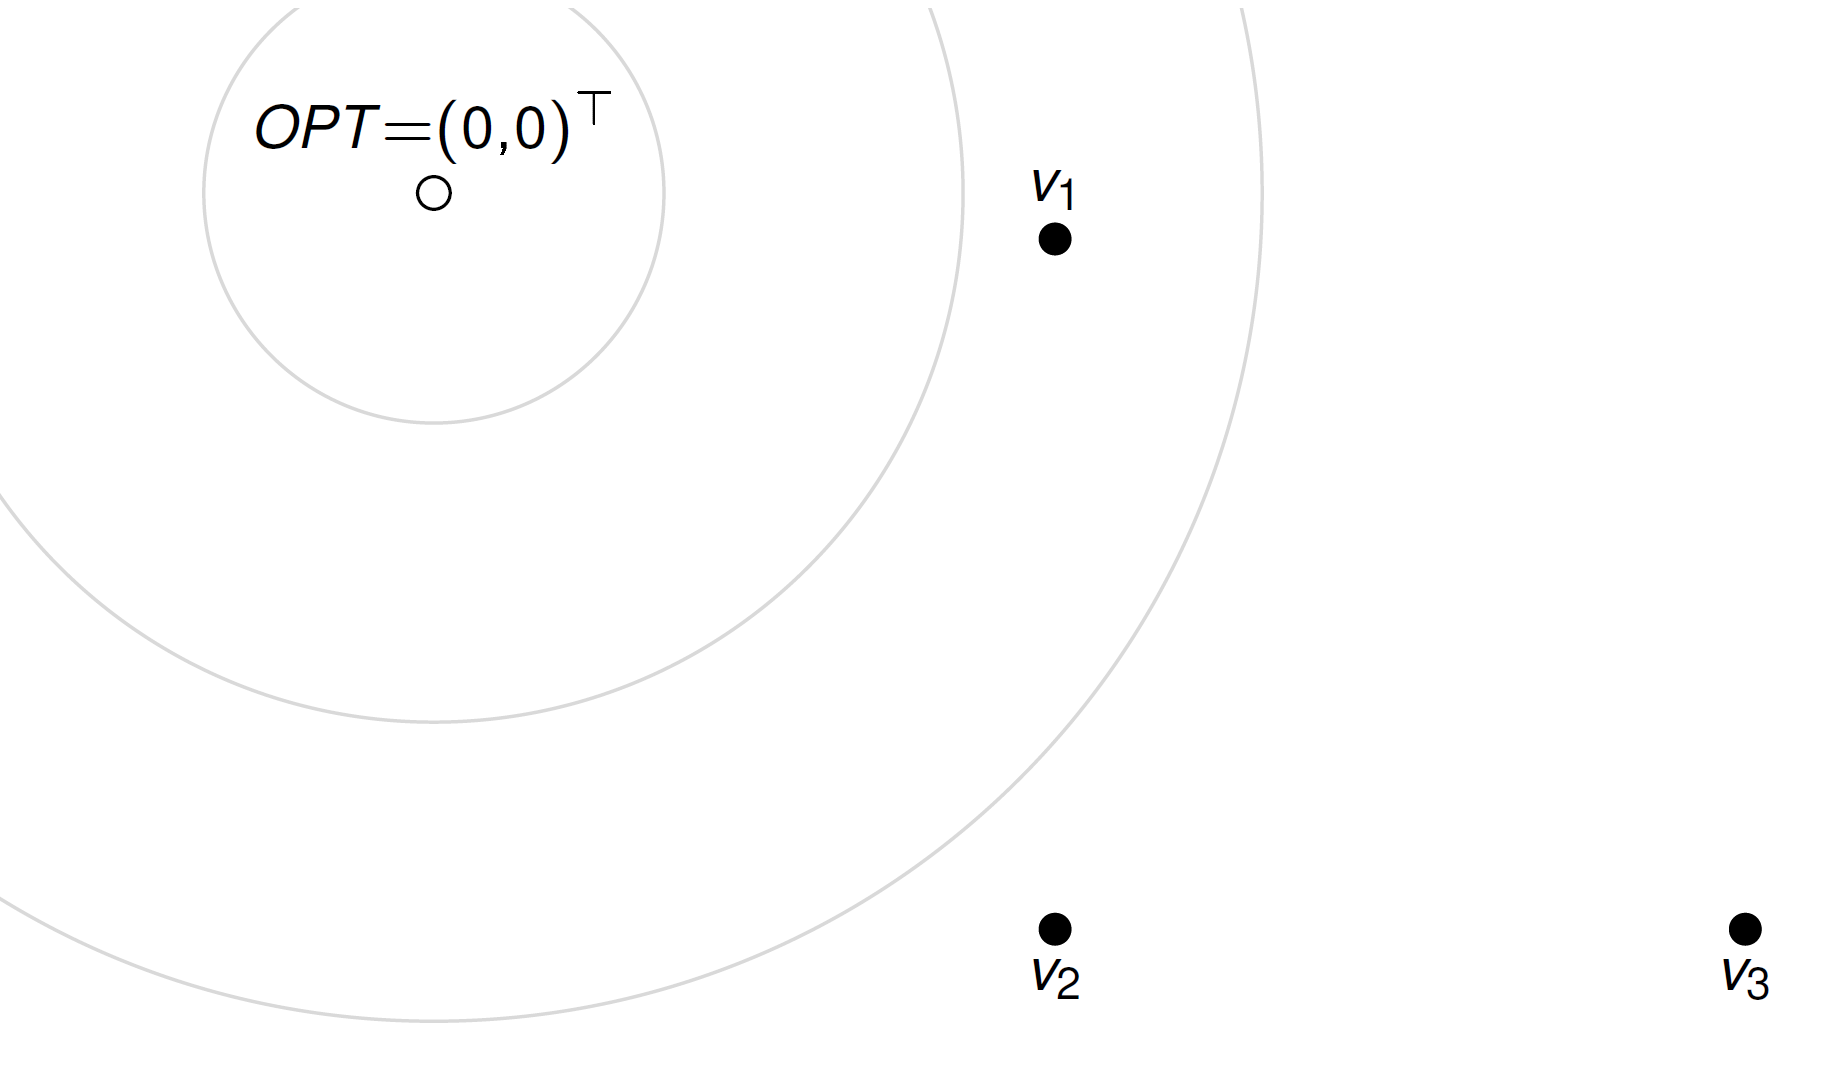
\includegraphics[width = 0.5\linewidth]{figure_man/Nelder01.png}
\end{figure}

\item Compute \textbf{centroid} without worst point
$$
\bar{\mathbf{v}} = \frac{1}{d} \sum_{i = 1}^d \mathbf{v}_i.
$$

\begin{figure}
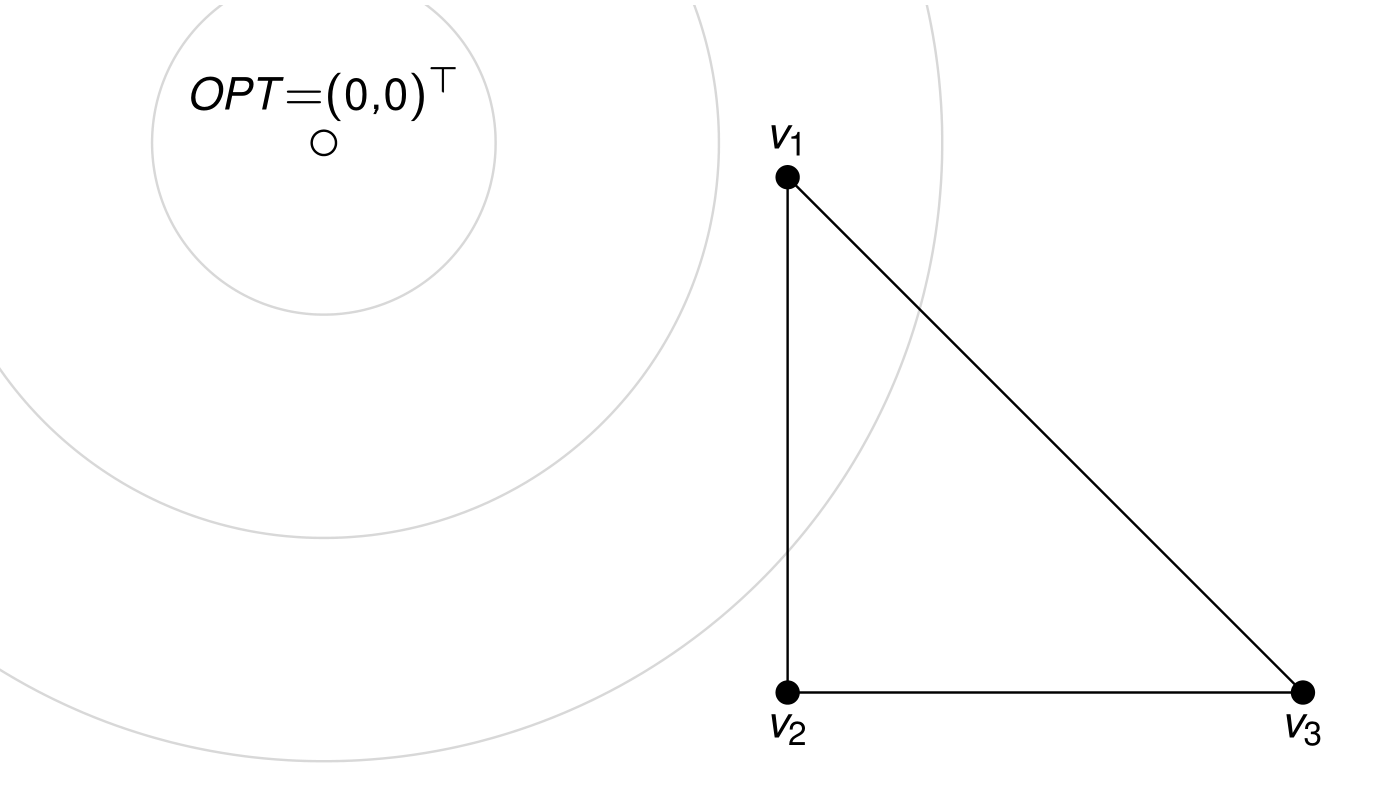
\includegraphics[width = 0.43\linewidth]{figure_man/Nelder02.png} ~~~ 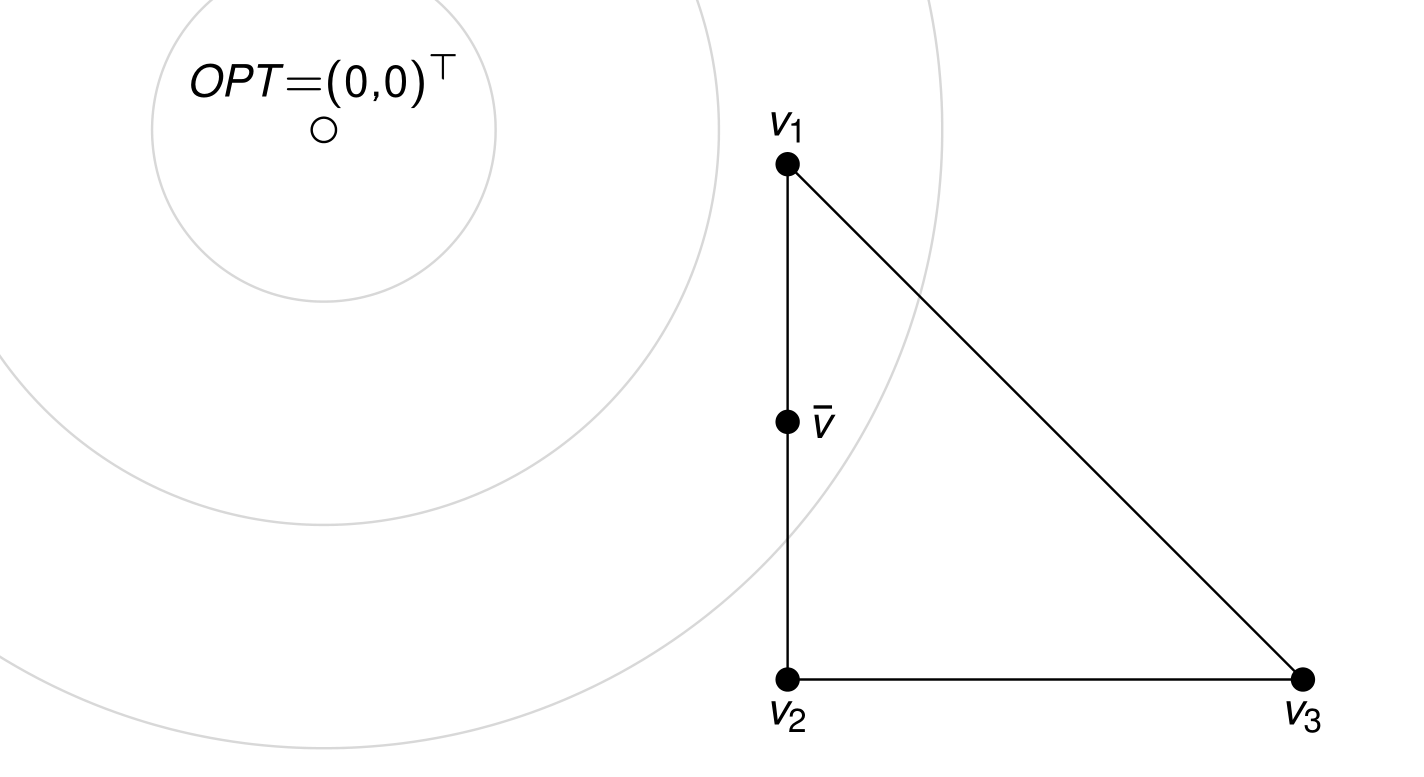
\includegraphics[width = 0.43\linewidth]{figure_man/Nelder03.png}
\end{figure}

\framebreak

\item \textbf{Reflection:} Compute reflection point
$$
\mathbf{v}_r = \bar{\mathbf{v}} + \rho (\bar{\mathbf{v}} - \mathbf{v}_{d + 1}),
$$
with $\rho > 0$.
Compute $f(\mathbf{v}_r)$.

\vspace{\baselineskip}

\begin{figure}
    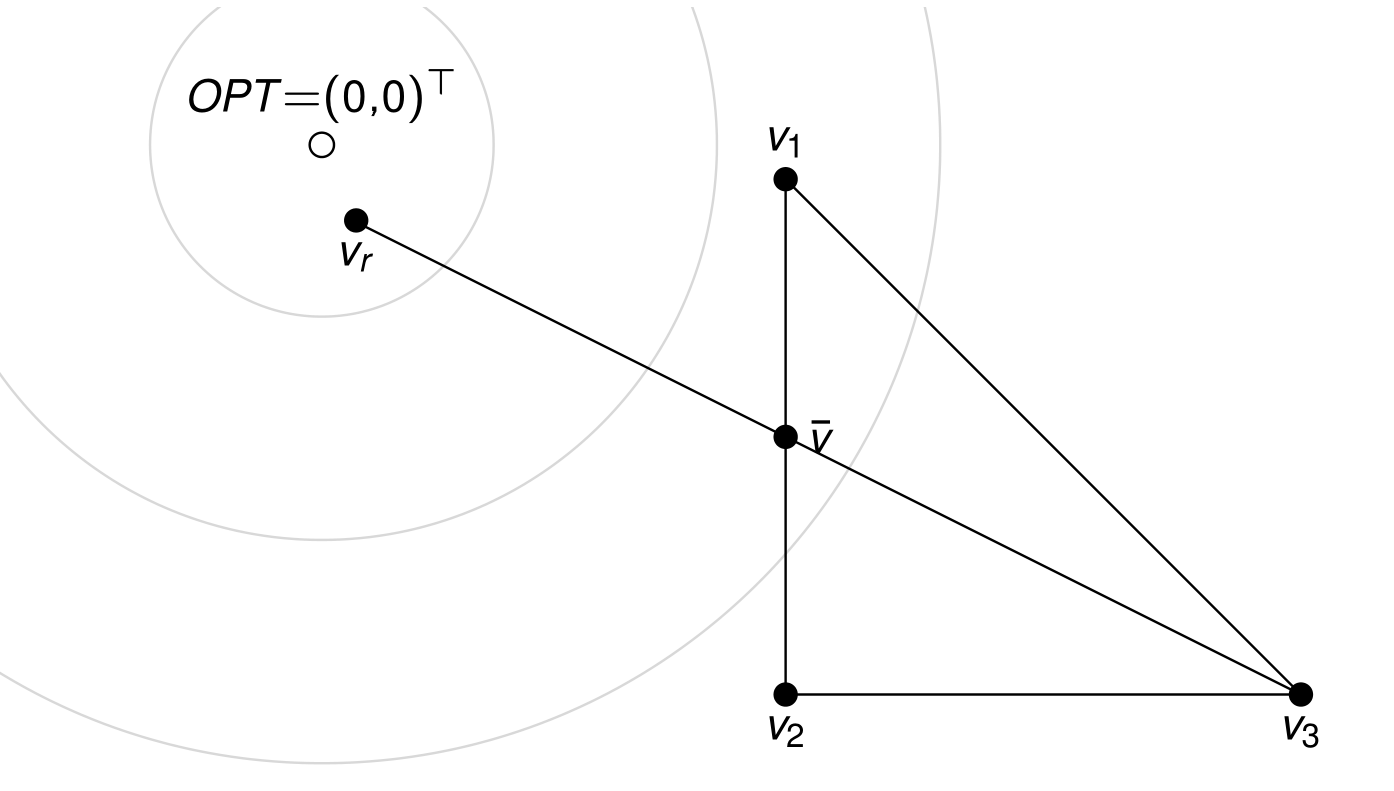
\includegraphics[width = 0.43\linewidth]{figure_man/Nelder04.png} 
\end{figure}

\vspace{\baselineskip}

\textbf{Note:} Default value for reflection coefficient: $\rho = 1$

\framebreak

\small
Distinguish three cases:

\begin{itemize}
    \small
    \item \textbf{Case 1:} $f(\mathbf{v}_1) \leq f(\mathbf{v}_r) < f(\mathbf{v}_d)$

        \medskip

        $\Rightarrow$ Accept $\mathbf{v}_r$ and discard $\mathbf{v}_{d + 1}$
\end{itemize}

%%%%%%%%%%%%%%%%%%%%%%%%%%%%%%%%%%
\medskip

\begin{minipage}{0.57\textwidth}
\begin{itemize}
    \small
    \item \textbf{Case 2:} $f(\mathbf{v}_r) < f(\mathbf{v}_1)$

        \medskip

        $\Rightarrow$ \textbf{Expansion:} 
        \begin{equation*}
            \mathbf{v}_e = \bar{\mathbf{v}} + \chi (\mathbf{v}_{r} - \bar{\mathbf{v}}), \quad \chi > 1.
        \end{equation*}
    
        We discard $\mathbf{v}_{d + 1}$ and except the better of $\mathbf{v}_r$ and $\mathbf{v}_e$.
\end{itemize}
\end{minipage}
\begin{minipage}{0.35\textwidth}
    \begin{center}
        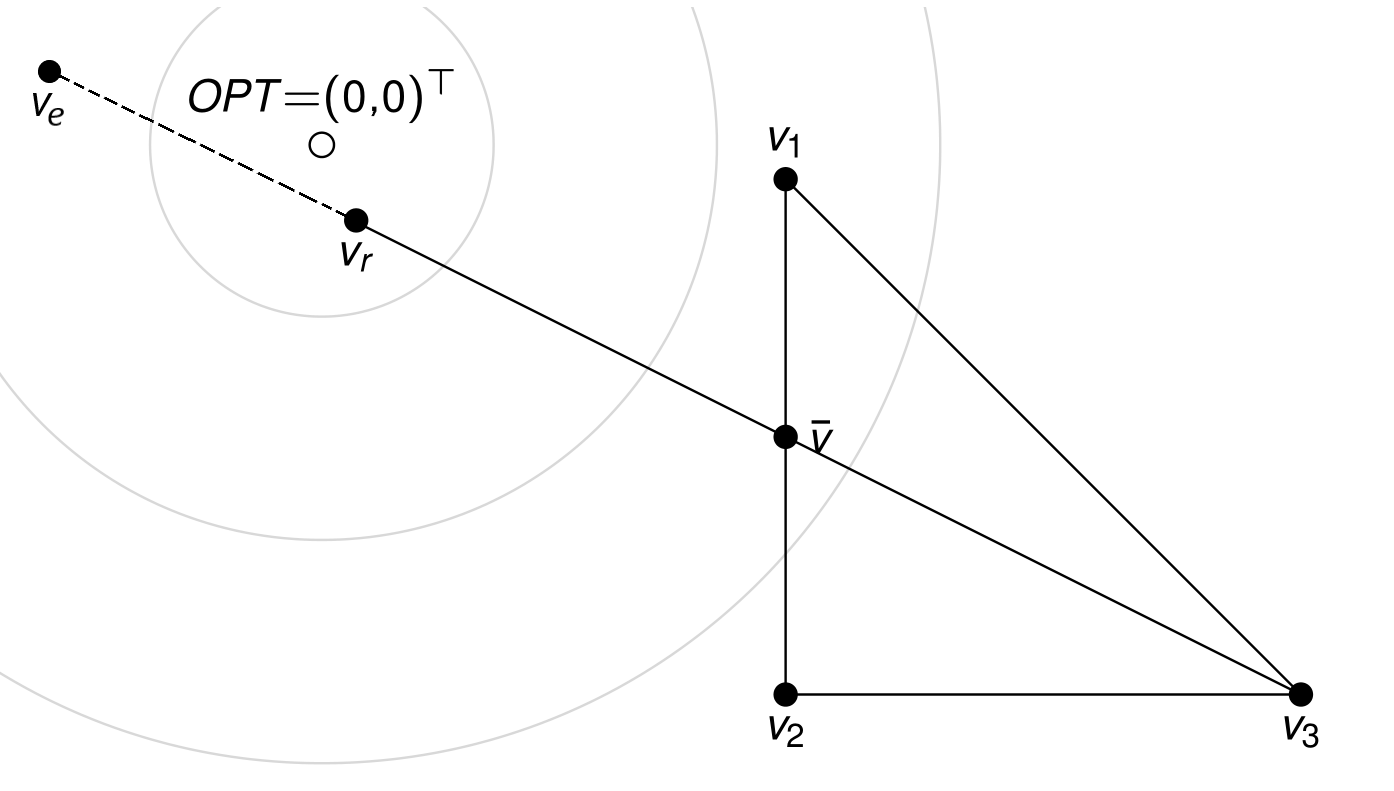
\includegraphics[width = 1\linewidth]{figure_man/Nelder06.png}
    \end{center}
\end{minipage}

\vspace{\baselineskip}

\textbf{Note:} Default value for expansion coefficient: $\chi = 2$

\framebreak

\begin{itemize}
    \small
    \item \textbf{Case 3:} $f(\mathbf{v}_r) \ge f(\mathbf{v}_d)$
        
        \medskip
        
        $\Rightarrow$ \textbf{Contraction:}
        \begin{equation*}
            \mathbf{v}_c = \bar{\mathbf{v}} + \gamma (\mathbf{v}_{d + 1} - \bar{\mathbf{v}})
        \end{equation*}
        with $0 < \gamma \le 1/2$.
        
        \begin{itemize}
            \item If $f(\mathbf{v}_c) < f(\mathbf{v}_{d + 1})$, accept $\mathbf{v}_c$.
            \item Otherwise, shrink \textbf{entire} simplex (\textbf{Shrinking}):
                \begin{equation*}
                    \mathbf{v}_{i} = \mathbf{v}_1 + \sigma (\mathbf{v}_{i} - \mathbf{v}_{1}) \quad \forall i
                \end{equation*}
        \end{itemize}

        \medskip
        
        \textbf{Note:} Default values for contraction and shrinking coefficient: $\gamma = \sigma = 1/2$
\end{itemize}

\item \textbf{Repeat} all steps until stopping criterion met.

\end{enumerate}

\end{vbframe}
%%%%%%%%%%%%%%%%%%%%%%%%%%%%%%%%%%%%%%%%%%%%%%%%%%%%%%%%%%%%%%%%%%%%%%%%%
%%%%%%%%%%%%%%%%%%%%%%%%%%%%%%%%%%%%%%%%%%%%%%%%%%%%%%%%%%%%%%%%%%%%%%%%%
%\framebreak
%A version of the \textbf{Nelder-Mead} method:

%\lz

%\textbf{Initialization:} Choose $p + 1$ random, linearly independent points $\mathbf{v}_i$ ($\mathbf{v}_i$ are vertices: corner points of the simplex/polytope):
%\begin{enumerate}
%\item \textbf{Order}: Order points according to ascending function values
%$$
%f(\mathbf{v}_1) \leq f(\mathbf{v}_2) \leq \ldots \leq f(\mathbf{v}_p) \leq f(\mathbf{v}_{p + 1}).
%$$
%with $\mathbf{v}_1$ best point, $\mathbf{v}_{p + 1}$ worst point.
%\item Calculate \textbf{centroid} without worst point
%$$
%\bar{\mathbf{v}} = \frac{1}{p} \sum_{i = 1}^p \mathbf{v}_i.
%$$
%\item \textbf{Reflection:} calculate reflection point
%$$
%\mathbf{v}_r = \bar{\mathbf{v}} + \rho (\bar{\mathbf{v}} - \mathbf{v}_{p + 1}),
%$$
%with $\rho > 0$. Calculate $f(\mathbf{v}_r)$.

%\framebreak

%We now distinguish three cases:

%\begin{itemize}
%\item \textbf{Case 1}: $f(\mathbf{v}_1) \leq f(\mathbf{v}_r) < f(\mathbf{v}_p)$ \\
%If the reflection point is better than the second worst corner, but not better than the best corner, we accept $\mathbf{v}_r$ and discard $\mathbf{v}_{p + 1}$.
%\vspace*{0.2cm}
%\item \textbf{Case 2}: $f(\mathbf{v}_r) < f(\mathbf{v}_1)$ \\
%If the reflection point is better than the best corner so far, we \enquote{expand} the current point (\textbf{Expansion}) to find out if we could get even better in the direction of $\mathbf{v}_r$:

%  $$
%  \mathbf{v}_e = \bar{\mathbf{v}} + \chi (\mathbf{v}_{r} - \bar{\mathbf{v}}), \quad \chi > 1.
%  $$

%We discard $\mathbf{v}_{p + 1}$ in favor of the better of the two corners $\mathbf{v}_r, \mathbf{v}_e$.
%\item \textbf{Case 3}: $f(\mathbf{v}_r) \ge f(\mathbf{v}_p)$
%we find that running toward $\mathbf{v}_{r}$ was not purposeful.
%We calculate a \textbf{contraction} point:

%$$
%\mathbf{v}_c = \bar{\mathbf{v}} + \gamma (\mathbf{v}_{p + 1} - \bar{\mathbf{v}})
%$$

%with $0 < \gamma \le 0.5$.
%\begin{itemize}
%\item If $\mathbf{v}_c$ is better than the worst point, we accept $\mathbf{x}_c$.
%\item Otherwise, we shrink the \textbf{entire} Simplex (\textbf{Shrinking}):

%$$
%\mathbf{v}_{i} = \mathbf{v}_1 + 0.5 (\mathbf{v}_{i} - \mathbf{v}_{1}) \quad \text{ for all } i
%$$
%\end{itemize}
%\end{itemize}

%In each of the three cases, we then continue with step 1 until a termination criterion is met.

%\end{enumerate}

%\end{vbframe}

%\begin{frame}[t, fragile]
%\frametitle{{Example: Nelder-Mead method}}
%  \begin{figure}[htbp]
%    \centering
%    \begin{tikzpicture}
%      \clip (-4.6,4) rectangle (6,-4);

      % Definiere Koordinaten
%      \coordinate (A) at (0,0);
%      \coordinate (B) at (3,0);
%      \coordinate (C) at (0,3);
%      \coordinate (D) at (-4,-2);
%      \coordinate (S) at (0,1.5);
%      \coordinate (K) at (-2.5,2.76);
%      \coordinate (OPT) at (-2.7,3.2);

%      \draw[gray!40] (OPT) circle (1cm);
%      \draw[gray!40] (OPT) circle (2.3cm);
%      \draw[gray!40] (OPT) circle (3.6cm);

        % Zeichne Ecken des Simplex mit Labels
%        \only<1>{\fill (A) circle (0.2em)};
%        \only<1>{\fill (B) circle (0.2em)};
%        \only<1>{\fill (C) circle (0.2em)};
%        \only<1-3>{\node[anchor=north,text width=12 cm] (note1) at (1.2,-0.5) {\scriptsize
%          \begin{enumerate}
%          \item \textbf{Order}: Order points by ascending function values
%          \setlength{\abovedisplayskip}{4pt}
%          \setlength{\belowdisplayskip}{4pt}
%          $$
%          f(\mathbf{v}_1) \leq f(\mathbf{v}_2) \leq \ldots \leq f(\mathbf{v}_p) \leq f(\mathbf{v}_{p + 1}).
%          $$
%          with $f(\mathbf{v}_1)$ as best point, $f(\mathbf{v}_{p + 1})$ as worst point.
%          \item Calculate \textbf{centroid} without worst point
%          $$
%          \bar{\mathbf{v}} = \frac{1}{p} \sum_{i = 1}^p \mathbf{v}_i.
%          $$
%          \end{enumerate}
%          };
%          \normalsize}

%        \only<4-5>{\node[anchor=north,text width=11 cm] (note2) at (1,-0.5) {\scriptsize
%          \begin{enumerate}\addtocounter{enumi}{2}
%          \item \textbf{Reflection:} calculate reflection point
%          \setlength{\abovedisplayskip}{4pt}
%          \setlength{\belowdisplayskip}{4pt}
%          $$
%          \mathbf{v}_r = \bar{\mathbf{v}} + \rho (\bar{\mathbf{v}} - \mathbf{v}_{p + 1}),
%          $$
%          with $\rho = 1$, calculate $f(\mathbf{v}_r)$.
%          \end{enumerate}
%          This is \textbf{case 2}: The reflection point $\mathbf{v}_r$ is better than the best point $\mathbf{v}_1$.\\
%        If the \textbf{expansion} does not return a better point than $\mathbf{v}_r$, accept $\mathbf{v}_r$ and reject $\mathbf{v}_3$.
%          };
%          \normalsize}

%      \fill<1-4> (A) circle (0.2em) node[below] {$\scriptstyle{v_{2}}$};
%      \only<1-4>{\fill (B) circle (0.2em) node[below] {$\scriptstyle{v_{3}}$};}
%      \fill<1-4> (C) circle (0.2em) node[above] {$\scriptstyle{v_{1}}$};
%      \only<3-4>{\fill (S) circle (0.2em) node[right] {$\scriptstyle{\bar{v}}$};}
%      \only<4>{\fill (K) circle (0.2em) node[below] {$\scriptstyle{v_{r}}$};}
%      \draw (OPT) circle (0.2em) node[above] {$\scriptstyle{OPT = (0,0)^{\top}}$};

      % Zeichne initiales Simplex
%      \only<2-4>{\draw (A) -- (C) -- (B) -- cycle;}

      % Zeichne Reflektionsgerade
%      \only<4>{\draw($(B)!-0cm!(S)$)--($(S)!-2.75cm!(B)$);}

      % Zeichne gestrichelt die Verbindungslinien zwischen den Ecken des neuen Simplex
%      \only<5->{
%      \draw (A) -- (C);
%      \draw[dashed] (C) -- (K) -- (A);
%      \fill (A) circle (0.2em) node[below] {$\scriptstyle{v_{3}}$};
%      \fill (C) circle (0.2em) node[above] {$\scriptstyle{v_{2}}$};
%      \fill (K) circle (0.2em) node[below] {$\scriptstyle{v_{1}}$};
%      }

%    \end{tikzpicture}
%    \lz
    %\caption{Erste (vereinfachte) Iteration Nelder-Mead Algo für Zielfunktion $f(x) = x_1^2 + x_2^2$ mit $x = (x_1, x_2)^{\top} \in \R^2$.}
%  \end{figure}
%\end{frame}
%%%%%%%%%%%%%%%%%%%%%%%%%%%%%%%%%%%%%%%%%%%%%%%%%%%%%%%%%%%%%%%%%%%%%
\begin{vbframe}{Nelder-Mead}
\small

\textbf{Advantages:}
\begin{itemize}
    \item No gradients needed
    \item Robust, often works well for non-differentiable functions.
\end{itemize}
\textbf{Drawbacks:}
\begin{itemize}
    \item Relatively slow (not applicable in high dimensions)
    \item Not each step improves solution, only mean of corner values is reduced.
    \item No guarantee for convergence to local optimum / stationary point.
\end{itemize}

\textbf{Visualization:}
\begin{center}
    \url{http://www.benfrederickson.com/numerical-optimization/}
\end{center}

\vspace{0.3cm}
\textbf{Note:} Nelder-Mead is default method of \texttt{R} function \texttt{optim()}.
If gradient is available and cheap, L-BFGS is preferred.

\end{vbframe}


\begin{frame}{Nelder-Mead Visualization in 2D}

$$\min_\xv f(x_1,x_2) = x_1^{2} + x_2^{2} + x_1\cdot \sin x_2 + x_2 \cdot \sin x_1 $$ 


\only<1>{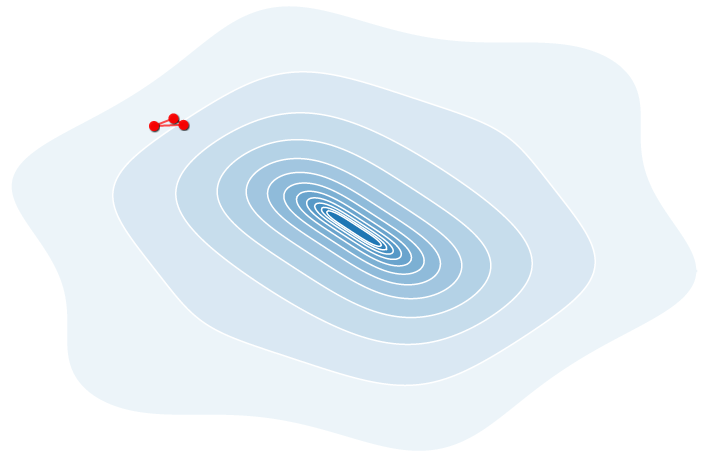
\includegraphics{figure_man/nm_animation2d_1.PNG}}
\only<2>{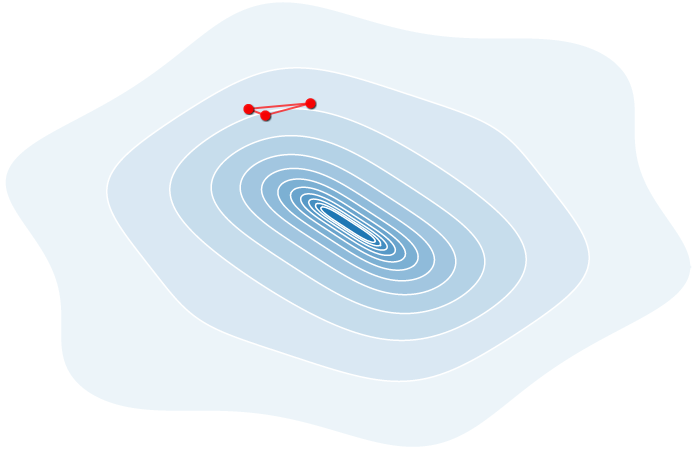
\includegraphics{figure_man/nm_animation2d_2.PNG}}
\only<3>{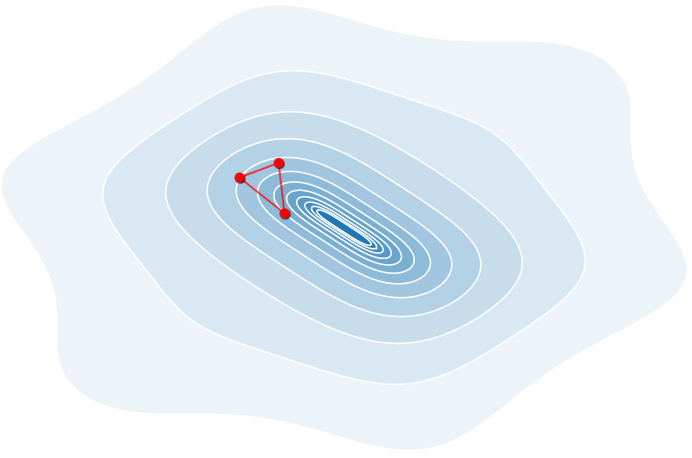
\includegraphics{figure_man/nm_animation2d_3.PNG}}
\only<4>{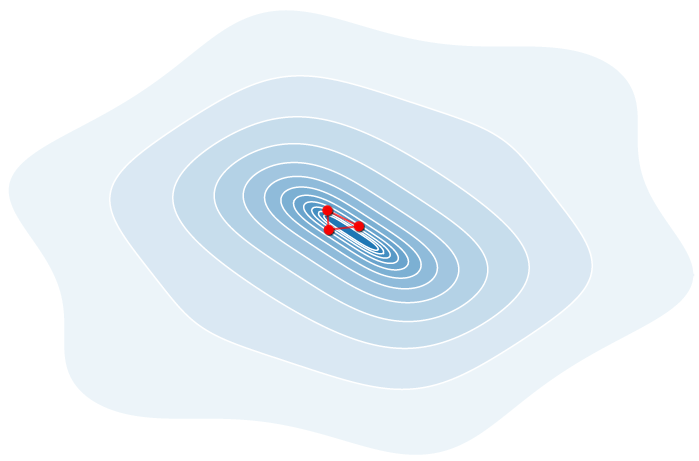
\includegraphics{figure_man/nm_animation2d_4.PNG}}

\end{frame}



\begin{vbframe}{Nelder-Mead vs. GD}
%% http://www.benfrederickson.com/numerical-optimization/
\vspace*{-0.5cm}
\begin{figure}
    \centering
    \begin{minipage}{0.45\textwidth}
        \centering
        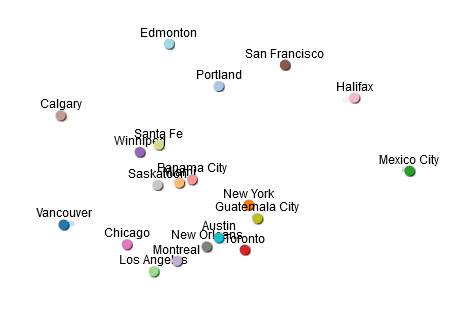
\includegraphics[width = 0.8\linewidth]{figure_man/nm_gd_cities_1.PNG}
    \end{minipage}\hfill
    \begin{minipage}{0.45\textwidth}
        \centering
        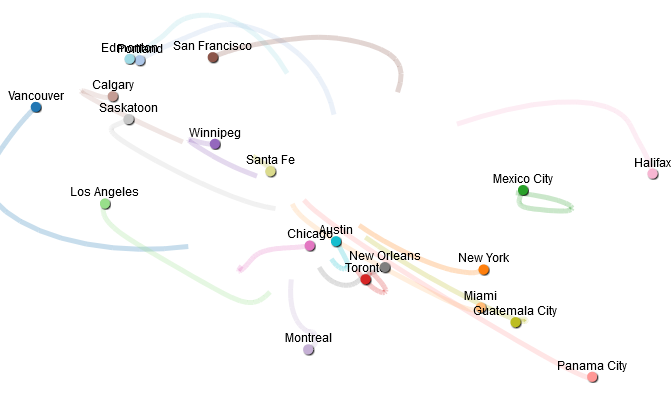
\includegraphics[width = 0.8\linewidth]{figure_man/nm_gd_cities_2.PNG}
    \end{minipage}
\end{figure}
\begin{figure}
    \centering
    \begin{minipage}{0.45\textwidth}
        \centering
        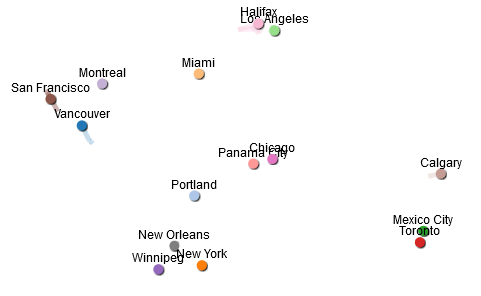
\includegraphics[width = 0.8\linewidth]{figure_man/nm_gd_cities_3.PNG}
    \end{minipage}\hfill
    \begin{minipage}{0.45\textwidth}
        \centering
        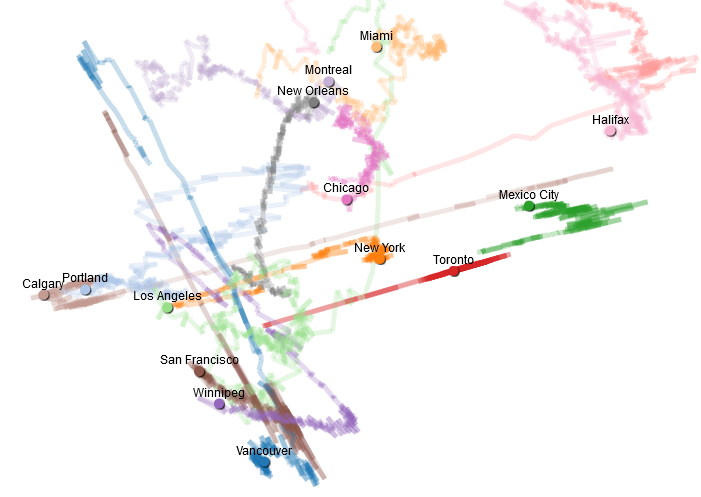
\includegraphics[width = 0.8\linewidth]{figure_man/nm_gd_cities_4.PNG}
    \end{minipage}
\end{figure}

\begin{footnotesize}
    Nelder-Mead in multiple dimensions:
    Organize points (US cities) to keep predefined mutual distances.
    For 10 cities, gradient descent (top) converges well for a suitable learning rate.
    Nelder-Mead (bottom) fails to converge, even after many iterations.
\end{footnotesize}


\framebreak
\vspace*{-0.8cm}
\begin{figure}
    \centering
    \begin{minipage}{0.45\textwidth}
        \centering
        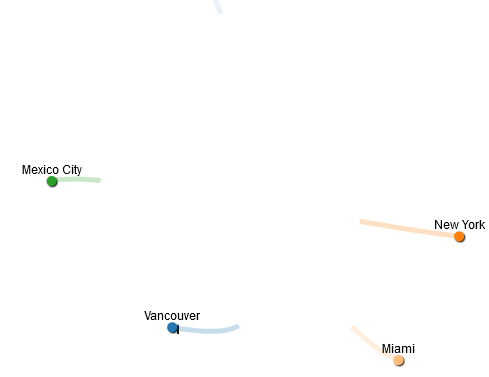
\includegraphics[width = 0.8\linewidth]{figure_man/nm_gd_cities_5.PNG}
    \end{minipage}\hfill
    \begin{minipage}{0.45\textwidth}
        \centering
        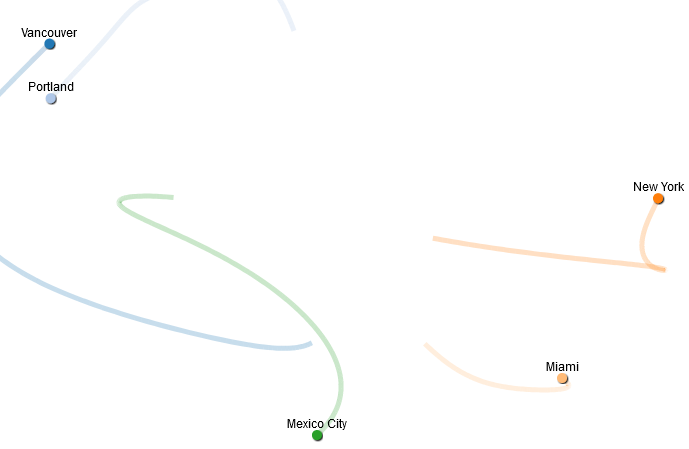
\includegraphics[width = 0.8\linewidth]{figure_man/nm_gd_cities_6.PNG}
    \end{minipage}
\end{figure}
\begin{figure}
    \centering
    \begin{minipage}{0.45\textwidth}
        \centering
        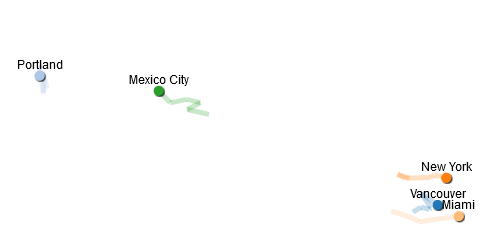
\includegraphics[width = 0.8\linewidth]{figure_man/nm_gd_cities_7.PNG}
    \end{minipage}\hfill
    \begin{minipage}{0.45\textwidth}
        \centering
        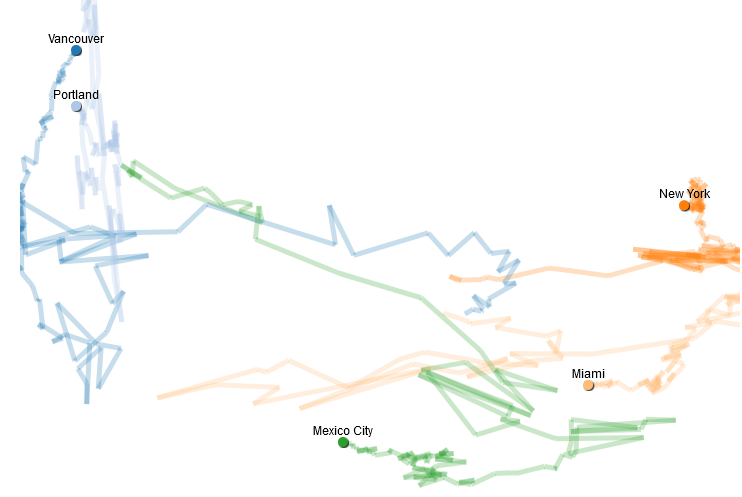
\includegraphics[width = 0.8\linewidth]{figure_man/nm_gd_cities_8.PNG}
    \end{minipage}
\end{figure}
\vspace*{0.5cm}
\begin{footnotesize}
    Even for only 5 cities, Nelder-Mead (bottom) performs poorly.
    However, gradient descent (top) still works.
\end{footnotesize}

\end{vbframe}



% \begin{vbframe}{Beispiel: MLE Gamma-Verteilung}
% \begin{itemize}
% \item Sei $x_1, \ldots, x_n$ zufälliges Sample einer $Gamma(r,\lambda)$ Verteilung ($r$ ist \textit{shape}, $\lambda$ \textit{rate} Parameter)
% \item $\theta = (r, \lambda) \in \R^2, \; \Theta = \R^+ \times \R^+$
% \item gesucht ist Maximum Likelihood Schätzer von $\theta$
% \end{itemize}
% $$
% L(r, \lambda) =  \frac{\lambda^{nr}}{\Gamma(r)^n} \prod_{i=1}^n x_i^{r-1} \exp(-\lambda \sum_{i=1}^nx_i), \; \; x_i \geq 0
% $$
% $$
% l(r, \lambda) = nr \log \lambda - n \log \Gamma(r) + (r-1) \sum_{i=1}^n \log x_i - \lambda \sum_{i=1}^n x_i
% $$

% \framebreak

% Direktes Maximieren von $l(r, \lambda)$ ist zweidimensionales Optimierungsproblem, alternativ kann univariates Nullstellenproblem über partielle Ableitungen formuliert werden.
% $$
% \frac{\partial}{\partial \lambda}l(r, \lambda)= \frac{nr}{\lambda}- \sum_{i=1}^n
% x_i = 0
% $$
% $$
% \frac{\partial}{\partial r}l(r, \lambda)=n \log \lambda - n \frac{\Gamma'(r)}{\Gamma(r)}+\sum_{i=1}^n \log x_i = 0
% $$
% Aus erster Gleichung folgt $\hat{\lambda} = \hat{r}/\bar{x}$. Setze $\hat{\lambda}$ für $\lambda$ in zweite Gleichung führt zu Nullstellensuche:
% $$
% n \log \frac{\hat{r}}{\bar{x}}+ \sum_{i=1}^n \log{x_i} - n \frac{\Gamma'(\hat{r})}{\Gamma(\hat{r})} = 0
% $$
% \framebreak
% \begin{itemize}
% \item Im Folgenden wird Optimierung per univariater Nullstellensuche und Nelder-Mead  durchgeführt
% \item 20000 mal 200 ZVZ aus $Gamma(r=5, \lambda=2)$ ziehen und Parameter schätzen
% \end{itemize}
% <<size = "scriptsize">>=
% # Univariate Nullstellensuche
% m = 20000; est_univ = matrix(0, m, 2); n = 200
% r = 5; lambda = 2
% # define objective function
% obj = function(lambda, xbar, logx.bar) {
%   digamma(lambda * xbar) - logx.bar - log(lambda)
% }

% for (i in 1:m) {
%   x = rgamma(n, shape = r, rate = lambda)
%   xbar = mean(x)
%   u = uniroot(obj, lower = .001, upper = 10e5,
%                xbar = xbar, logx.bar = mean(log(x)))
%   lambda.hat = u$root
%   r.hat = xbar * lambda.hat
%   est_univ[i, ] = c(r.hat, lambda.hat)
% }
% MLU = colMeans(est_univ)
% @

% <<size = "scriptsize">>=
% # optim Nelder-Nead
% LL = function(theta, sx, slogx, n) {
%   r = theta[1]
%   lambda = theta[2]
%   loglik = n * r * log(lambda) + (r - 1) * slogx -
%     lambda * sx - n * log(gamma(r))
%   - loglik
% }

% n = 200; r = 5; lambda = 2

% est_nelder = replicate(20000, expr = {
%   x = rgamma(200, shape = 5, rate = 2)
%   optim(c(1,1), LL, sx = sum(x), slogx = sum(log(x)), n = n)$par
% })
% MLN = rowMeans(est_nelder)
% @

% <<echo=FALSE>>=
% par(mfrow=c(2,2))
% hist(est_univ[, 1], breaks="scott", freq=FALSE,
%      xlab="r", main="Univariate")
% points(MLU[1], 0, cex=1.5, pch=20)
% hist(est_univ[, 2], breaks="scott", freq=FALSE,
%      xlab=bquote(lambda), main="Univariate")
% points(MLU[2], 0, cex=1.5, pch=20)

% hist(est_nelder[1,], breaks="scott", freq=FALSE,
%      xlab="r", main="Nelder-Mead")
% points(MLN[1], 0, cex=1.5, pch=20)
% hist(est_nelder[2,], breaks="scott", freq=FALSE,
%      xlab=bquote(lambda), main="Nelder-Mead")
% points(MLN[2], 0, cex=1.5, pch=20)
%@
% \end{vbframe}

% \section{Metaheuristiken}



% \begin{vbframe}{Simulated Annealing}
% Allgemeines Optimierungsverfahren aus dem Bereich des Machine
% Learnings, das auch bei unstetigen und diskreten Problemen
% Verwendung
% finden kann.

% \lz

% Name: {\em Annealing = Hartglühen} (Metallurgie)
% \begin{enumerate}
% \item Starte mit $\mathbf{x}^{(0)}$
% \item Ziehe zufällige Änderung $\epsilon$, setzte $\tilde{x} = \mathbf{x}^{(i)} + \eta^{(i)}\epsilon$
% \begin{itemize}
% \item $f(\tilde{x}) < f(\mathbf{x}^{(i)}) \Rightarrow \mathbf{x}^{(i + 1)} = \tilde{x}$
% \item $f(\tilde{x}) \ge f(\mathbf{x}^{(i)}) \Rightarrow \mathbf{x}^{(i + 1)} = \begin{cases}
% \tilde{x}  &\text{ mit Wkt.\ } p^{(i)}\\
% x_i  \ \ &\text{ mit Wkt.\ } 1 - p^{(i)}
% \end{cases}$
% \end{itemize}
% \item Wiederhole ab 2. bis zur maximalen Anzahl an Iterationen
% \end{enumerate}

% \lz

% \begin{tabular}{ll}
% $\eta^{(i)}, p^{(i)} \rightarrow 0$ & in Abhängigkeit von \enquote{Temperatur}. \\
% $\eta^{(i)}$ & Schrittweite in Iteration $i$ .\\
% $p^{(i)}$ & Wkt.\ Verschlechterung zu akzeptieren.
% \end{tabular}
% \end{vbframe}

\endlecture
\end{document}

